
\actTitle{Worksheet 3.1}

\noindent \textbf{Instructions:}  Work together in groups of  3 or 4 to complete the following problems.

Student goals:
\begin{itemize}
\item Determine if a given function is one-to-one. The function can
  be given in graphical, tabular, or algebraic forms.
\item Explicitly show that a function is one-to-one or demonstrate why
  a function is not one-to-one.
\item Determine the inverse of a given function. The function can be
  given in tabular or algebraic forms.
\item Determine the domain and range of the inverse of a function. The
  function can be given in graphical, tabular, or algebraic forms.
\item Limit the domain of a function that is not one-to-one so that an
  inverse can be defined on the resulting restricted domain.
\end{itemize}


For the following set of questions your group should work with three
functions that you will construct. You will start with three basic
functions and transform them into new functions which will be used
throughout the remaining questions.
\begin{enumerate}
\item Use $g(x)=x^2$ and two of the following functions for your
  group.  Along with $g(x)$ choose two from the following functions:
  $$f(x)=x, \quad \quad
  h(x)=x^3, \quad \quad
  j(x)=\frac{1}{x}, \quad \quad
  m(x)=\sqrt{x},  \quad \quad
  p(x)=\sqrt[3]{x}.$$

\item Pick some transformations like shifting, stretching,
  compressing, and reflecting to transform each of your 3
  functions. Give each of your new functions a new name and write your
  3 new functions below.  \sideNote{These are transformations for you
    to choose.}

  \vfill

\item Calculate the domain and range. For each of the 3 new functions.

  \vfill

\clearpage


\item Determine \emph{algebraically} if each of your functions are one-to-one.  

\vfill
\vfill


\item For each of your functions that are not one-to-one, make a
  domain restriction so that the function becomes one-to-one on the
  new domain.

\vfill

\clearpage


\item For each of your functions (including those with new domain restrictions), find their inverse functions.

\vfill

\item Use function composition to verify that the inverse functions you have described are truly inverses to your functions.

\vfill

\clearpage

\item Graph your function and its inverse on the same coordinate axes.  Check that they are properly symmetric to each other.

\begin{multicols}{2}

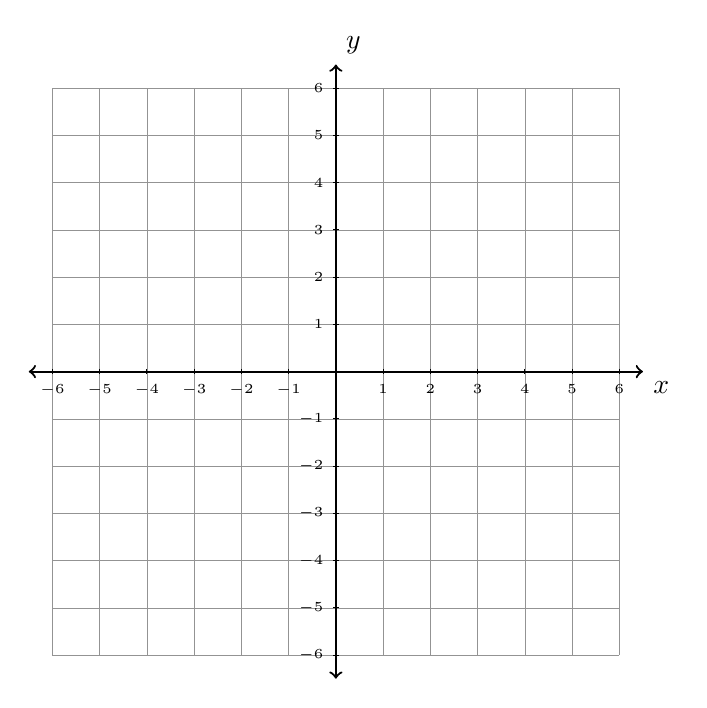
\begin{tikzpicture}[y=.6cm, x=.6cm,font=\sffamily,
	mydot/.style={
    circle,
    fill=white,
    draw,
    outer sep=0pt,
    inner sep=1.5pt
  }]
    %% Add a grid
    \draw[step = 1, gray, very thin,opacity=0.85] (-6, -6) grid (6, 6);
 	%% Draw the axes
	\draw[thick,<->] (-6.5,0) -- coordinate (x axis mid) (6.5,0) node[anchor = north west] {$x$};
    \draw[thick,<->] (0,-6.5) -- coordinate (y axis mid) (0,6.5) node[anchor = south west] {$y$};
    %% Label the y axis
    \foreach \y in {-6,...,-1,1,2,...,6} {
      \draw (1pt, \y) -- (-1pt, \y) node[anchor =  east] {\tiny$\y$};
    }
    %% Label the x axis
    \foreach \x in {-6,...,-1,1,2,...,6} {
      \draw (\x,1pt) -- (\x,-1pt) node[anchor = north] {\tiny$\x$};
    }
    %% Draw the function.
 %   \begin{scope}
 %        \draw[very thick,black] (-3,2) -- (1,1);
 %        \draw[very thick,black] (3.05,1.05) -- (4,3);
    %semi-circle
  %       \draw[very thick, black] (1,1) arc [radius=1, start angle=180, end angle= 5];
     %parabola
     %    \draw[ultra thick, black, domain=-5:0] plot (\x, {(-0.2)*(\x-5)*(\x+5)});
     %dots
     %  \fill[black] (-3, 2) circle[radius=0.5ex];
     %   \fill[black] (1,1) circle[radius=0.5ex];
     %    \fill[black] (4,3) circle[radius=0.5ex];
     %     \draw[very thick, black] (3,1) circle[radius=0.5ex];


   % \end{scope}

    %%\node[above=0.1cm] at (-2,2 )   {\nextXValue};

  \end{tikzpicture}

\vspace{1in}


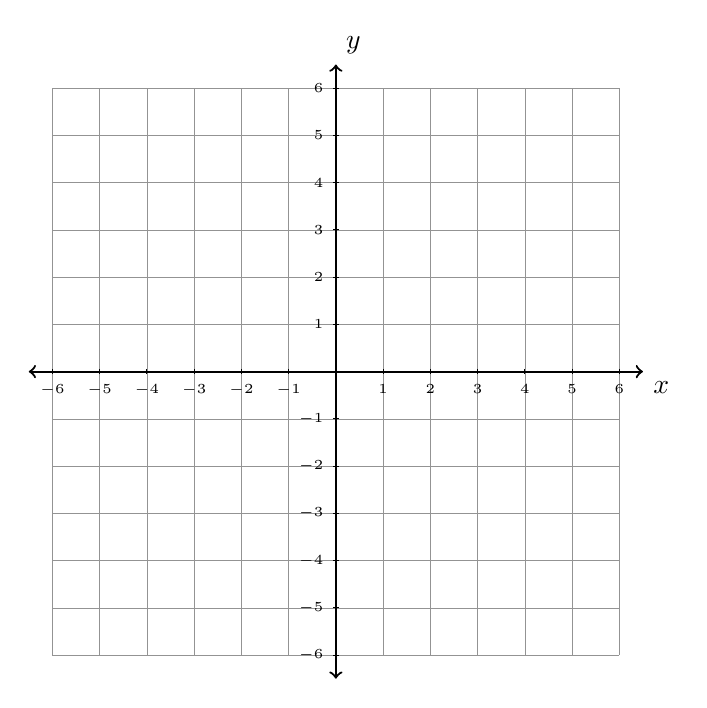
\begin{tikzpicture}[y=.6cm, x=.6cm,font=\sffamily,
	mydot/.style={
    circle,
    fill=white,
    draw,
    outer sep=0pt,
    inner sep=1.5pt
  }]
    %% Add a grid
    \draw[step = 1, gray, very thin,opacity=0.85] (-6, -6) grid (6, 6);
 	%% Draw the axes
	\draw[thick,<->] (-6.5,0) -- coordinate (x axis mid) (6.5,0) node[anchor = north west] {$x$};
    \draw[thick,<->] (0,-6.5) -- coordinate (y axis mid) (0,6.5) node[anchor = south west] {$y$};
    %% Label the y axis
    \foreach \y in {-6,...,-1,1,2,...,6} {
      \draw (1pt, \y) -- (-1pt, \y) node[anchor =  east] {\tiny$\y$};
    }
    %% Label the x axis
    \foreach \x in {-6,...,-1,1,2,...,6} {
      \draw (\x,1pt) -- (\x,-1pt) node[anchor = north] {\tiny$\x$};
    }
    %% Draw the function.
 %   \begin{scope}
 %        \draw[very thick,black] (-3,2) -- (1,1);
 %        \draw[very thick,black] (3.05,1.05) -- (4,3);
    %semi-circle
  %       \draw[very thick, black] (1,1) arc [radius=1, start angle=180, end angle= 5];
     %parabola
     %    \draw[ultra thick, black, domain=-5:0] plot (\x, {(-0.2)*(\x-5)*(\x+5)});
     %dots
     %  \fill[black] (-3, 2) circle[radius=0.5ex];
     %   \fill[black] (1,1) circle[radius=0.5ex];
     %    \fill[black] (4,3) circle[radius=0.5ex];
     %     \draw[very thick, black] (3,1) circle[radius=0.5ex];


   % \end{scope}

    %%\node[above=0.1cm] at (-2,2 )   {\nextXValue};

  \end{tikzpicture}



\columnbreak

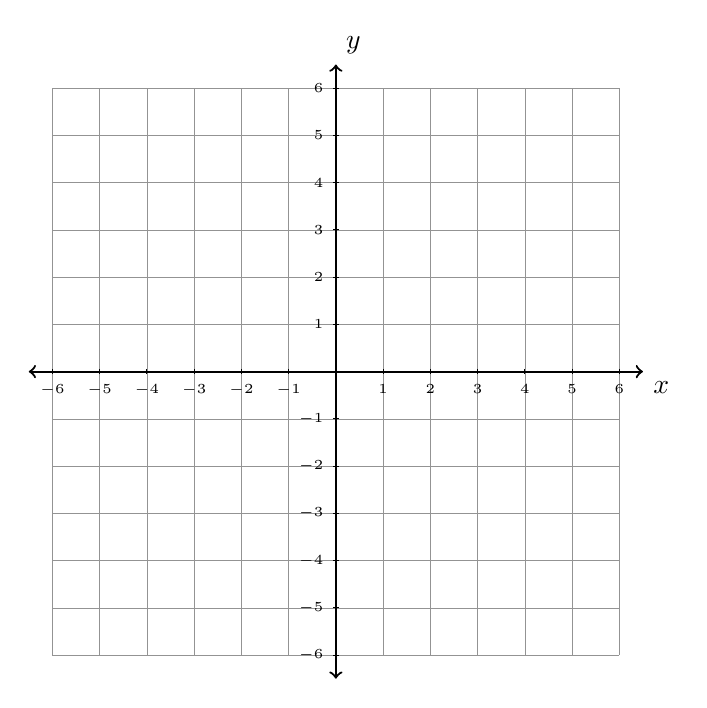
\begin{tikzpicture}[y=.6cm, x=.6cm,font=\sffamily,
	mydot/.style={
    circle,
    fill=white,
    draw,
    outer sep=0pt,
    inner sep=1.5pt
  }]
    %% Add a grid
    \draw[step = 1, gray, very thin,opacity=0.85] (-6, -6) grid (6, 6);
 	%% Draw the axes
	\draw[thick,<->] (-6.5,0) -- coordinate (x axis mid) (6.5,0) node[anchor = north west] {$x$};
    \draw[thick,<->] (0,-6.5) -- coordinate (y axis mid) (0,6.5) node[anchor = south west] {$y$};
    %% Label the y axis
    \foreach \y in {-6,...,-1,1,2,...,6} {
      \draw (1pt, \y) -- (-1pt, \y) node[anchor =  east] {\tiny$\y$};
    }
    %% Label the x axis
    \foreach \x in {-6,...,-1,1,2,...,6} {
      \draw (\x,1pt) -- (\x,-1pt) node[anchor = north] {\tiny$\x$};
    }
    %% Draw the function.
 %   \begin{scope}
 %        \draw[very thick,black] (-3,2) -- (1,1);
 %        \draw[very thick,black] (3.05,1.05) -- (4,3);
    %semi-circle
  %       \draw[very thick, black] (1,1) arc [radius=1, start angle=180, end angle= 5];
     %parabola
     %    \draw[ultra thick, black, domain=-5:0] plot (\x, {(-0.2)*(\x-5)*(\x+5)});
     %dots
     %  \fill[black] (-3, 2) circle[radius=0.5ex];
     %   \fill[black] (1,1) circle[radius=0.5ex];
     %    \fill[black] (4,3) circle[radius=0.5ex];
     %     \draw[very thick, black] (3,1) circle[radius=0.5ex];


   % \end{scope}

    %%\node[above=0.1cm] at (-2,2 )   {\nextXValue};

  \end{tikzpicture}
  

\vspace{1in}


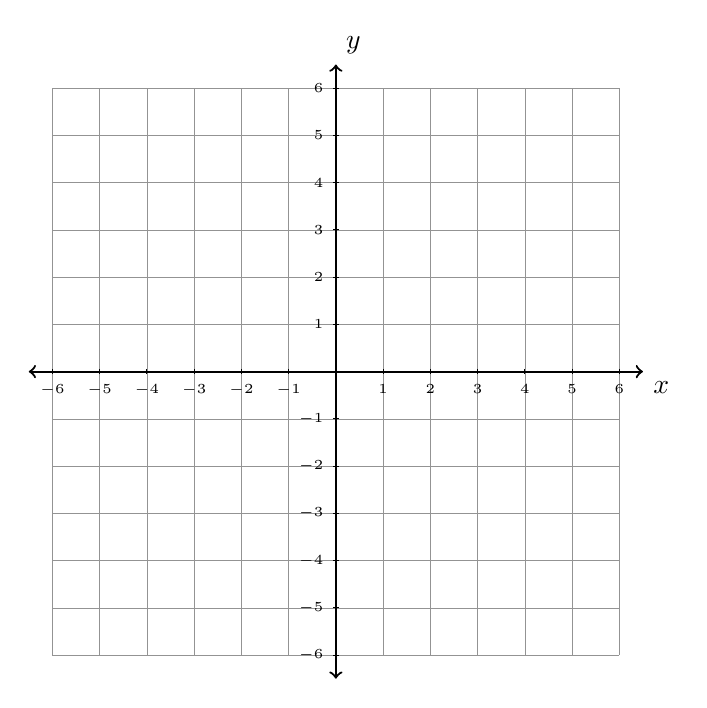
\begin{tikzpicture}[y=.6cm, x=.6cm,font=\sffamily,
	mydot/.style={
    circle,
    fill=white,
    draw,
    outer sep=0pt,
    inner sep=1.5pt
  }]
    %% Add a grid
    \draw[step = 1, gray, very thin,opacity=0.85] (-6, -6) grid (6, 6);
 	%% Draw the axes
	\draw[thick,<->] (-6.5,0) -- coordinate (x axis mid) (6.5,0) node[anchor = north west] {$x$};
    \draw[thick,<->] (0,-6.5) -- coordinate (y axis mid) (0,6.5) node[anchor = south west] {$y$};
    %% Label the y axis
    \foreach \y in {-6,...,-1,1,2,...,6} {
      \draw (1pt, \y) -- (-1pt, \y) node[anchor =  east] {\tiny$\y$};
    }
    %% Label the x axis
    \foreach \x in {-6,...,-1,1,2,...,6} {
      \draw (\x,1pt) -- (\x,-1pt) node[anchor = north] {\tiny$\x$};
    }
    %% Draw the function.
 %   \begin{scope}
 %        \draw[very thick,black] (-3,2) -- (1,1);
 %        \draw[very thick,black] (3.05,1.05) -- (4,3);
    %semi-circle
  %       \draw[very thick, black] (1,1) arc [radius=1, start angle=180, end angle= 5];
     %parabola
     %    \draw[ultra thick, black, domain=-5:0] plot (\x, {(-0.2)*(\x-5)*(\x+5)});
     %dots
     %  \fill[black] (-3, 2) circle[radius=0.5ex];
     %   \fill[black] (1,1) circle[radius=0.5ex];
     %    \fill[black] (4,3) circle[radius=0.5ex];
     %     \draw[very thick, black] (3,1) circle[radius=0.5ex];


   % \end{scope}

    %%\node[above=0.1cm] at (-2,2 )   {\nextXValue};

  \end{tikzpicture}
  
  
\end{multicols}

\clearpage

\item Determine whether or not each relationship below is a function.
  For each relationship that is a function briefly discuss whether or
  not it is a one-to-one function. Briefly explain your reasoning. if
  a function is not one-to-one determine a restriction on the domain
  so that it is one-to-one on the restricted domain.

  \begin{enumerate}
  \item ~ \\
  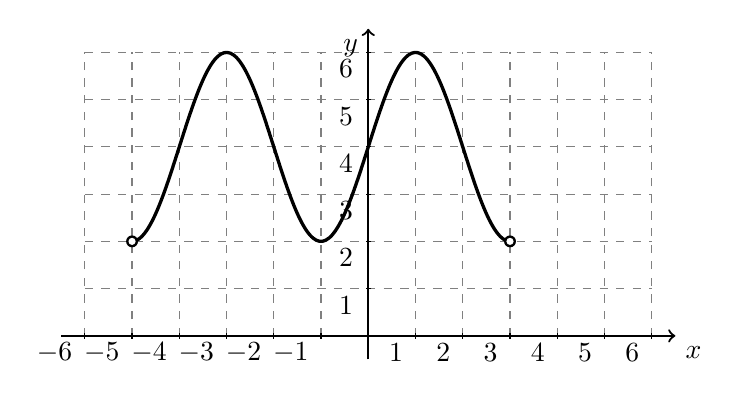
\begin{tikzpicture}[y=0.6cm, x=0.6cm,font=\sffamily]
    %% ticks
    \draw[step = 1, gray,dashed] (-6,0) grid (6,6);
    %% axis
    \draw[thick,->] (-6.5,0) -- coordinate (x axis mid) (6.5,0) node[anchor = north west] {$x$};
    \draw[thick,->] (0,-.5) -- coordinate (y axis mid) (0,6.5) node[anchor = north east] {$y$};
    \foreach \y in {1,2,...,6} {
      \draw (1pt, \y) -- (-1pt, \y) node[yshift=-6,xshift=-1,anchor=east] {$\y$};
    }
    \foreach \x in {-6,-5,...,-1,1,2,...,6} {
      \draw (\x,1pt) -- (\x,-1pt) node[yshift=-5,xshift=-1,anchor=east] {$\x$};
    }

    \begin{scope}
      %\clip(-4,-1) rectangle (8,5);
      \draw[scale=1.0,domain=-4:4,smooth,variable=\x,very thick,black,samples=120] 
           plot ({\x-1},{4+2*sin(deg(pi*\x/2-pi/2))});
      \fill[black] (-5,2) circle [radius=0.5ex];
      \fill[white] (-5,2) circle [radius=0.3ex];
      \fill[black] ( 3,2) circle [radius=0.5ex];
      \fill[white] ( 3,2) circle [radius=0.3ex];
    \end{scope}

  \end{tikzpicture}

  \vfill
  
  \item ~ \\
    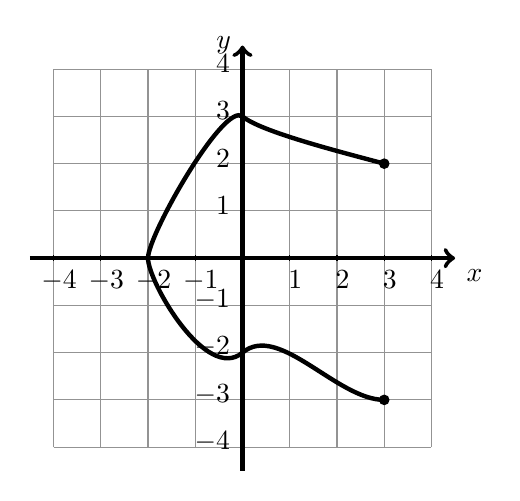
\begin{tikzpicture}[y=0.6cm, x=0.6cm,font=\sffamily]
      \draw[step = 1, gray, thin,opacity=0.85] (-4,-4) grid (4,4);
      \draw[black,ultra thick,->] (-4.5,0) -- (4.5,0) node[anchor=north west] {$x$};
      \draw[black,ultra thick,->] (0,-4.5) -- (0,4.5) node[anchor=east] {$y$};
      \foreach \y in {-4,-3,-2,-1,1,2,3,4} {
        \draw (1pt, \y) -- (-1pt, \y) node[anchor = east,yshift=2] {$\y$};
        \draw (\y,1pt) -- (\y,-1pt) node[anchor = north,xshift=2] {$\y$};
      }
      \draw[ultra thick,black] (3, -3) .. controls +(0:-1) and +(40:1) .. (0, -2)
                    ( 0,-2) .. controls +( 40:-1.0) and +(90:-0.5) .. (-2, 0)
                    (-2, 0) .. controls +( 90:0.5) and +(-40:-0.5) .. (0,3)
                    ( 0, 3) .. controls +(-40:0.5) and +(-15:-1) .. (3, 2);
          \draw[black,fill=black]  (3,-3) circle (0.1);
          \draw[black,fill=black]  (3, 2) circle (0.1);

    \end{tikzpicture}

    \vfill
    
    \item ~ \\
    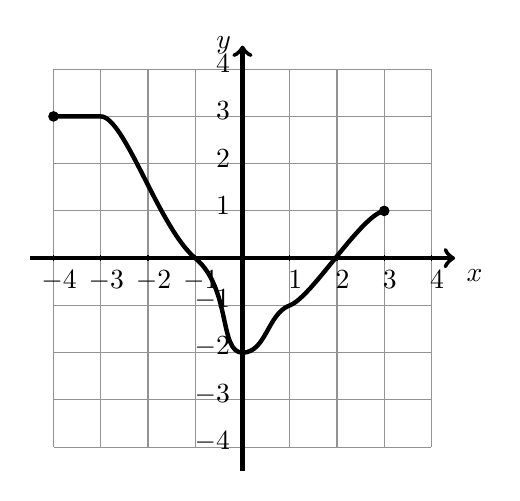
\begin{tikzpicture}[y=0.6cm, x=0.6cm,font=\sffamily]
      \draw[step = 1, gray, thin,opacity=0.85] (-4,-4) grid (4,4);
      \draw[black,ultra thick,->] (-4.5,0) -- (4.5,0) node[anchor=north west] {$x$};
      \draw[black,ultra thick,->] (0,-4.5) -- (0,4.5) node[anchor=east] {$y$};
      \foreach \y in {-4,-3,-2,-1,1,2,3,4} {
        \draw (1pt, \y) -- (-1pt, \y) node[anchor = east,yshift=2] {$\y$};
        \draw (\y,1pt) -- (\y,-1pt) node[anchor = north,xshift=2] {$\y$};
      }
      \draw[ultra thick,black]
                    (-4,3)  .. controls +(0:1) and +(180:0.5) .. (-3,3)
                    (-3, 3) .. controls +(0:0.5) and +(140:1) .. (-1, 0)
                    ( -1,0) .. controls +( 140:-1) and +(180:0.5) .. (0, -2)
                    ( 0, -2) .. controls +(0:0.5) and +(200:0.5) .. (1,-1)
                    ( 1, -1) .. controls +(200:-0.5) and  +(190:0.5) .. (3,1);
          \draw[black,fill=black]  (-4,3) circle (0.1);
          \draw[black,fill=black]  (3, 1) circle (0.1);

    \end{tikzpicture}

    \vfill
    
  \end{enumerate}

\end{enumerate}




